\Exhibit{AkvelonRsSalary}{%
    Ответ Налоговой службы Грузии о зарплате Алексея Инкина до вычета налогов, проверяемый online\WithTr%
}

Этот ответ Налоговой службы Грузии показывает зарплату до вычета налогов,
полученную Алексеем Инкиным, равную 167014.90 лари.

Этот ответ содержит QR-код, который отрывает этот же документ на сайте
Налоговой службы, таким образом подтверждая подлинность документа.

\begin{center}
    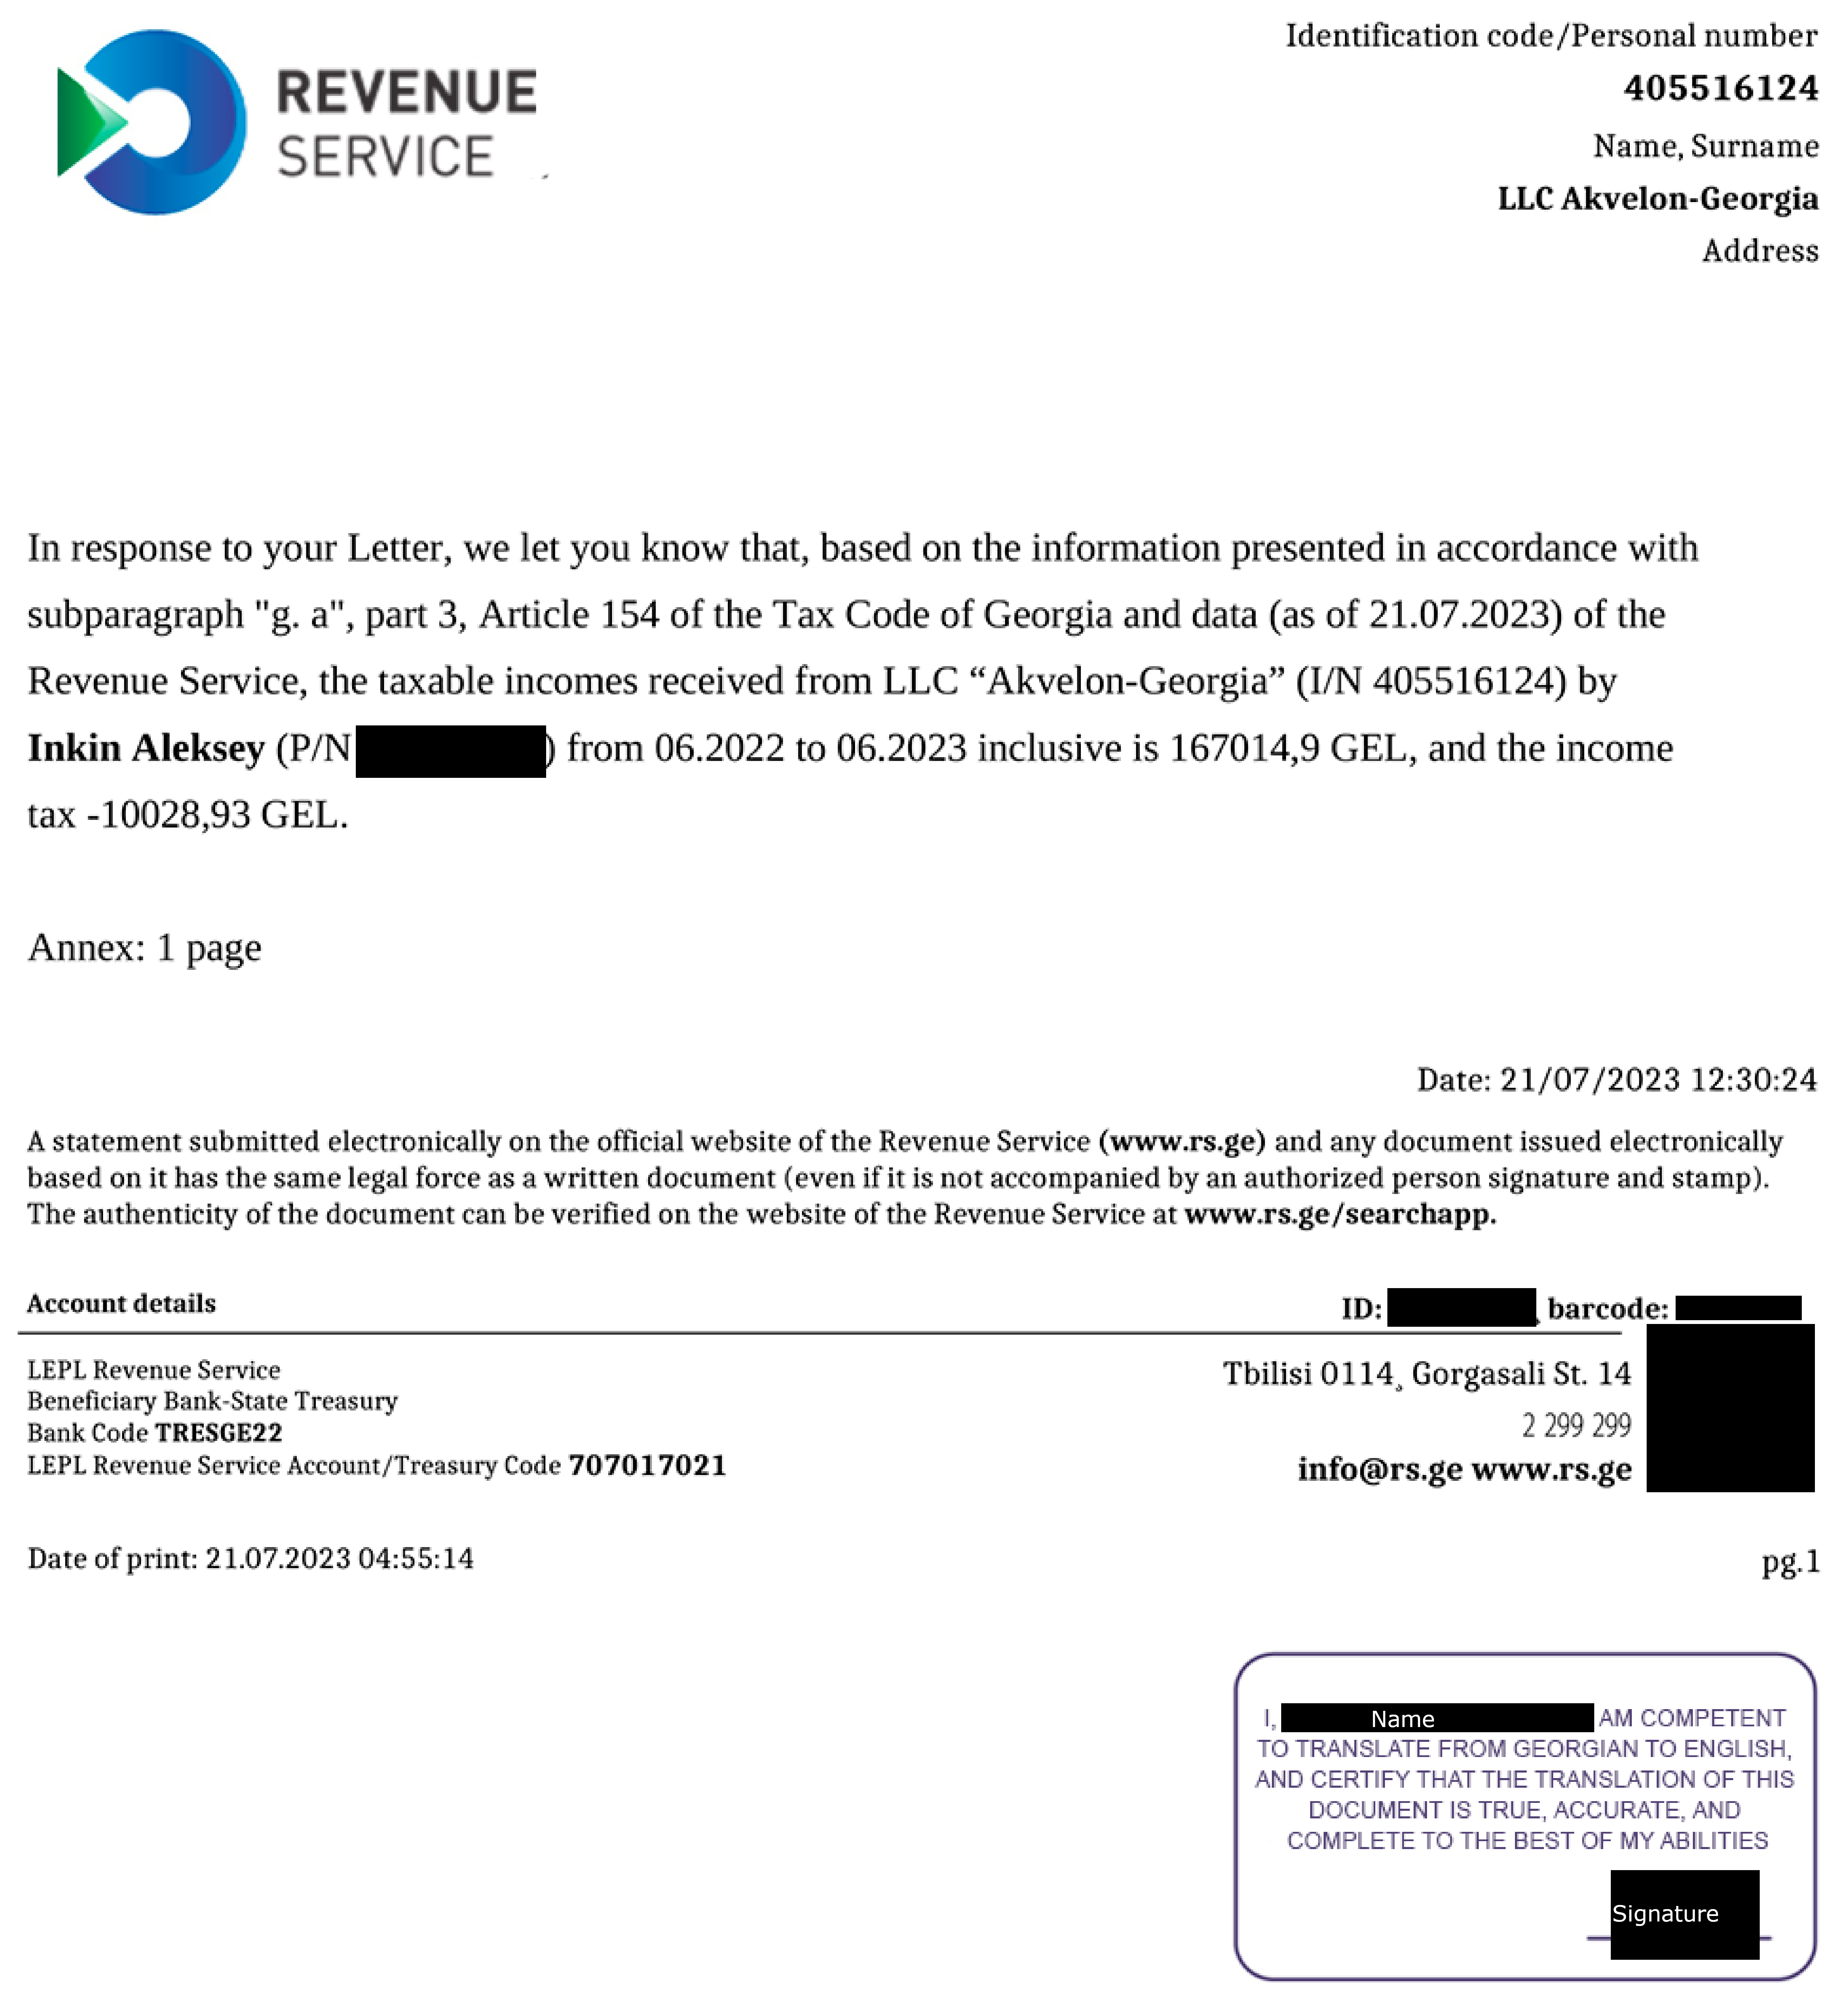
\includegraphics[width=35em]{rs-1_en_public}
\end{center}

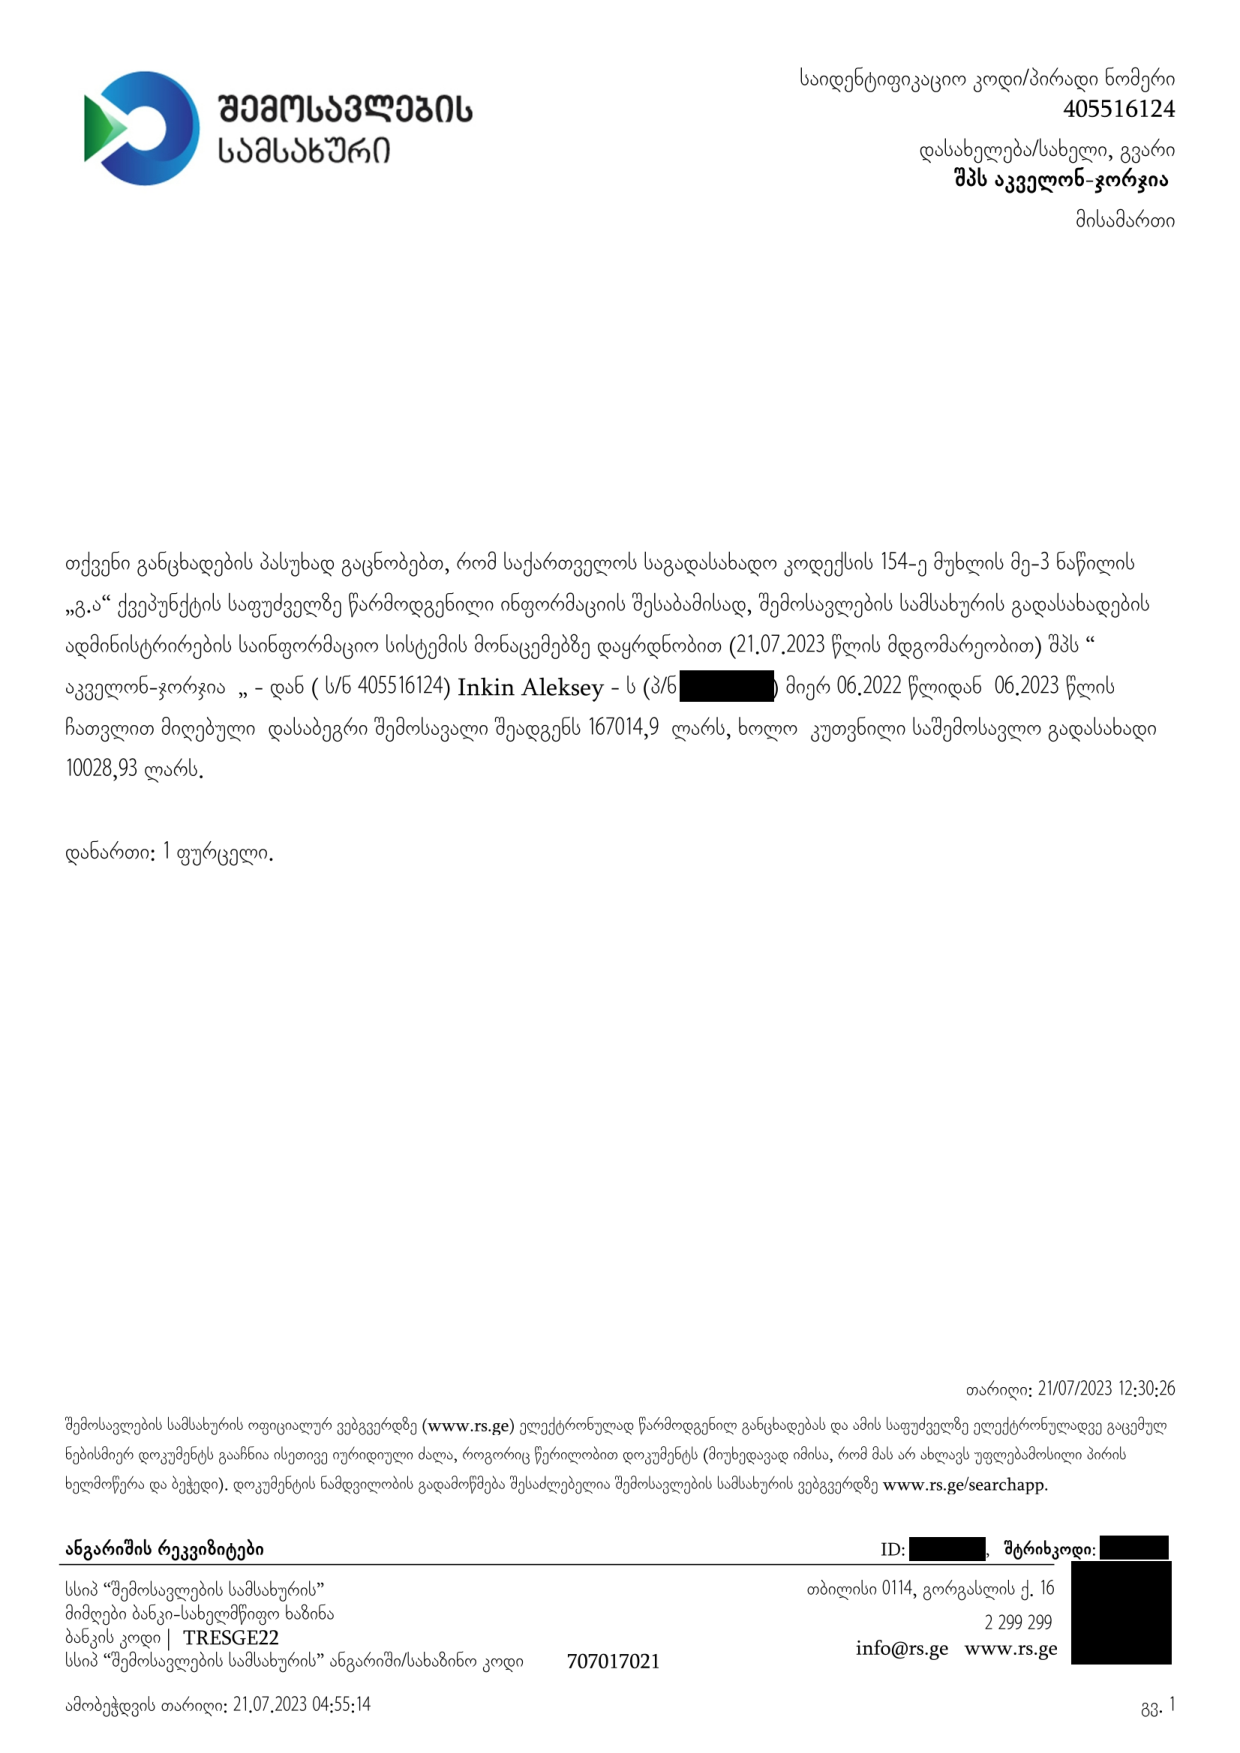
\includepdf[pages=-]{rs-1_public}

\begin{center}
    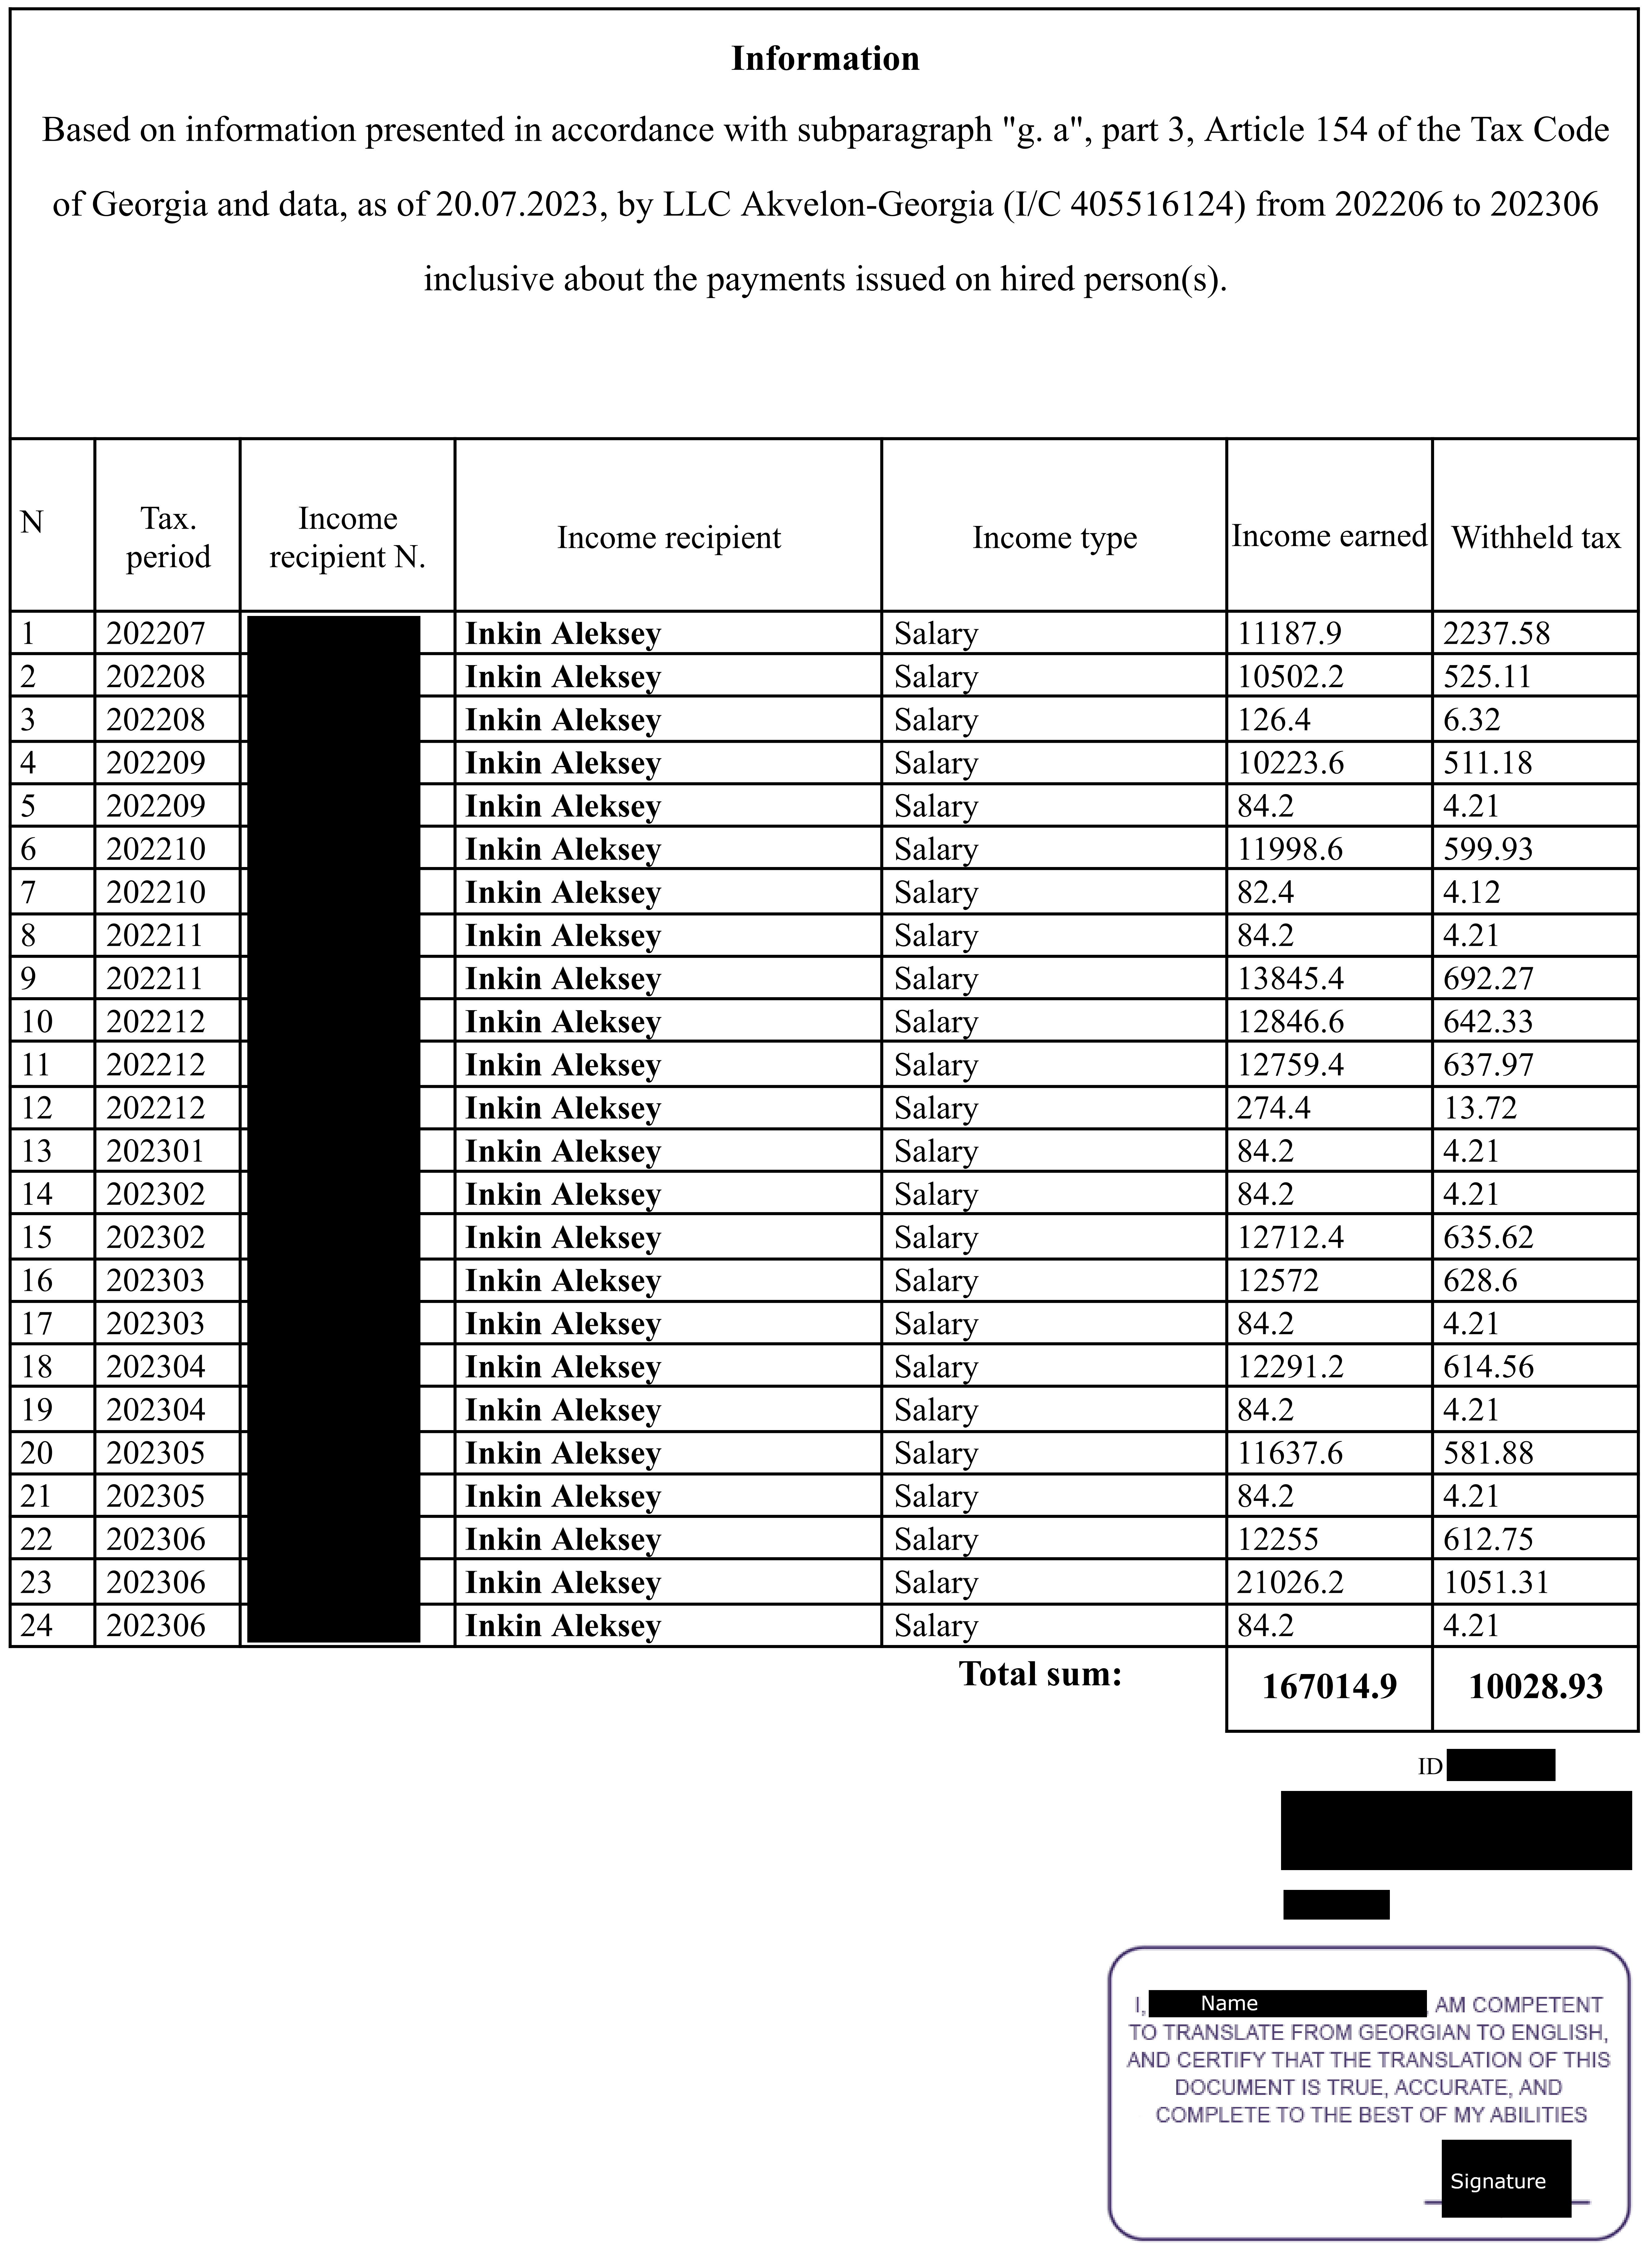
\includegraphics[width=35em]{rs-2_en_public}
\end{center}

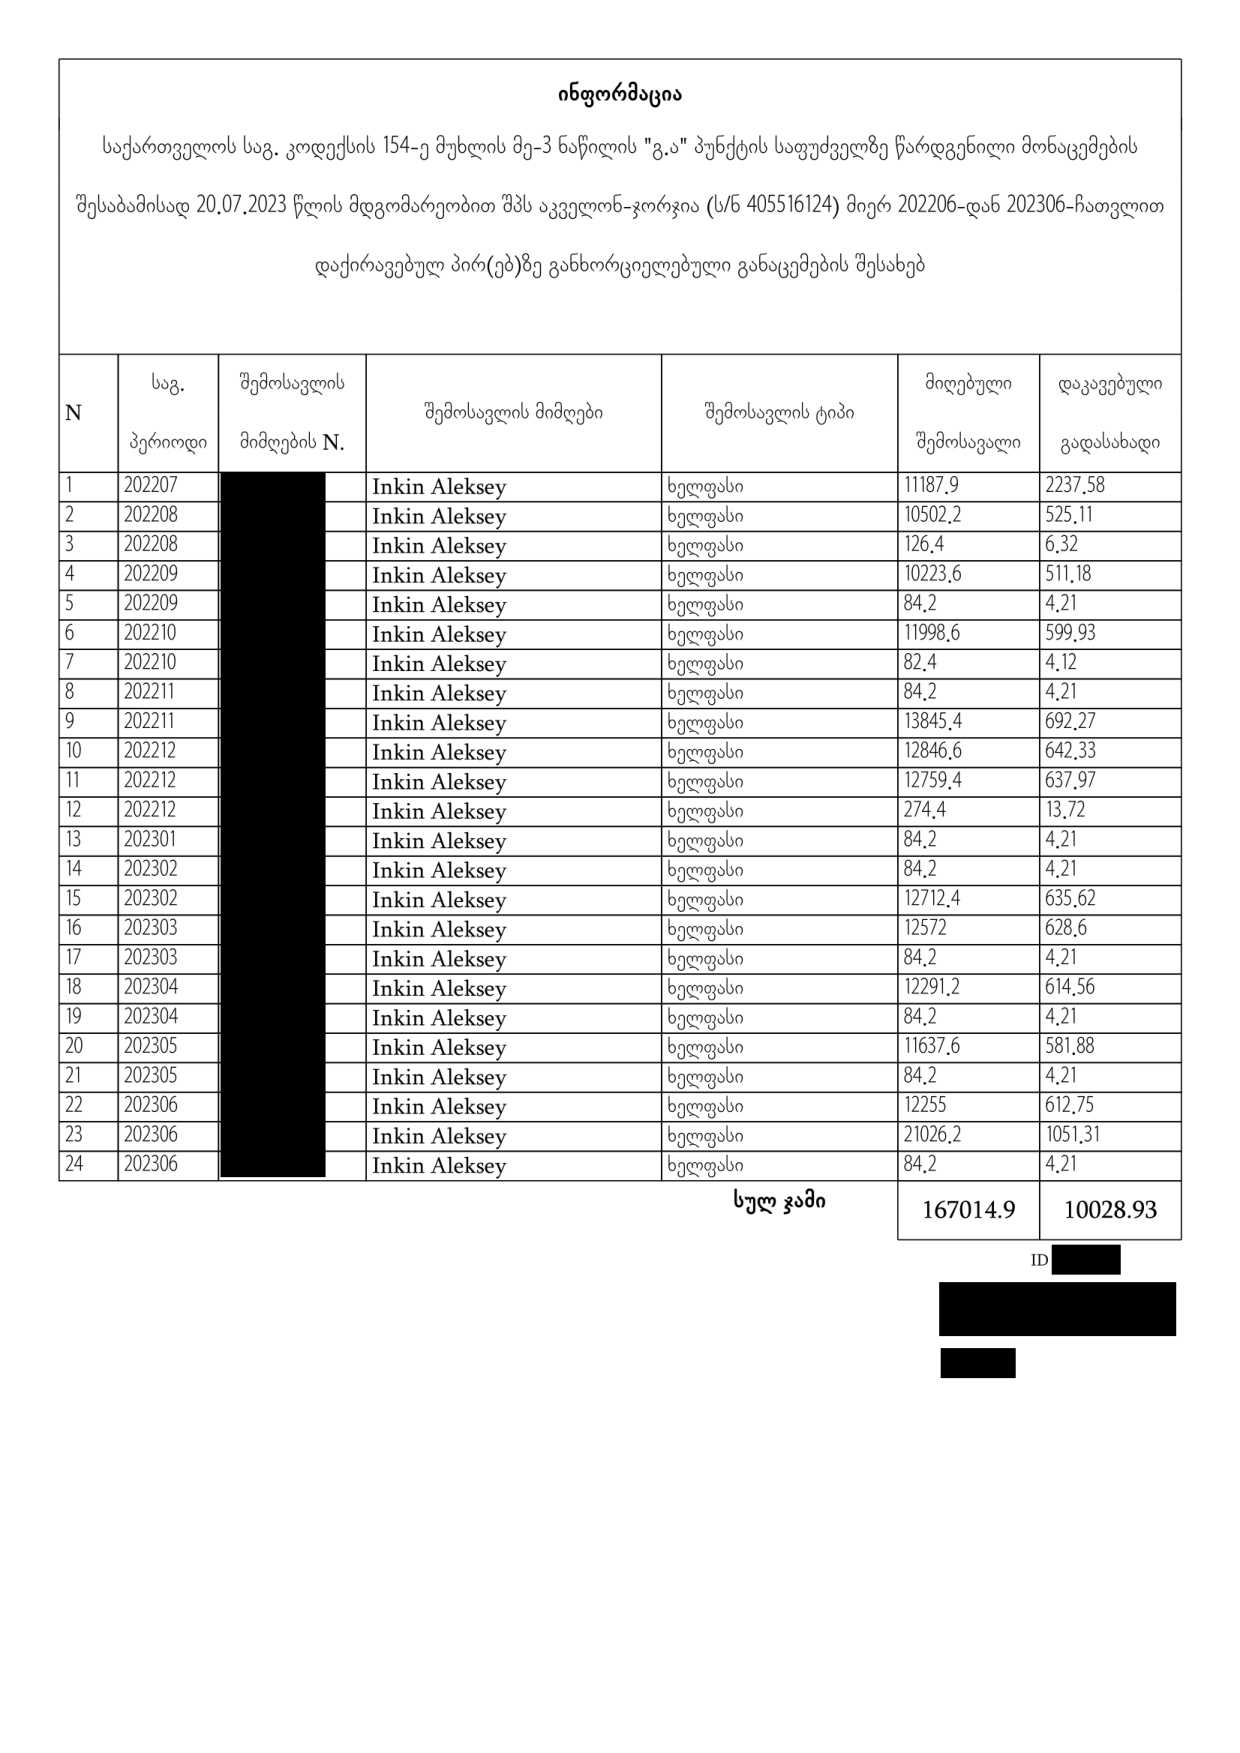
\includepdf[pages=-]{rs-2_public}

Другой способ проверить этот документ -- зайти на
https://www.rs.ge/searchapp

Эта страница запрашивает Application ID (первое поле)
и Barcode number (второе поле).
Введите следующее, как написано в документе:

\begin{tabular}{ll}
    Application ID: & <\dots> \\
    Barcode number: & <\dots> \\
\end{tabular}


Во всплывающем окне две кнопки, чтобы открыть две страницы ответа Налоговой службы.

\begin{center}
    \includegraphics[width=35em]{rs-verification_en_public}
\end{center}

\begin{center}
    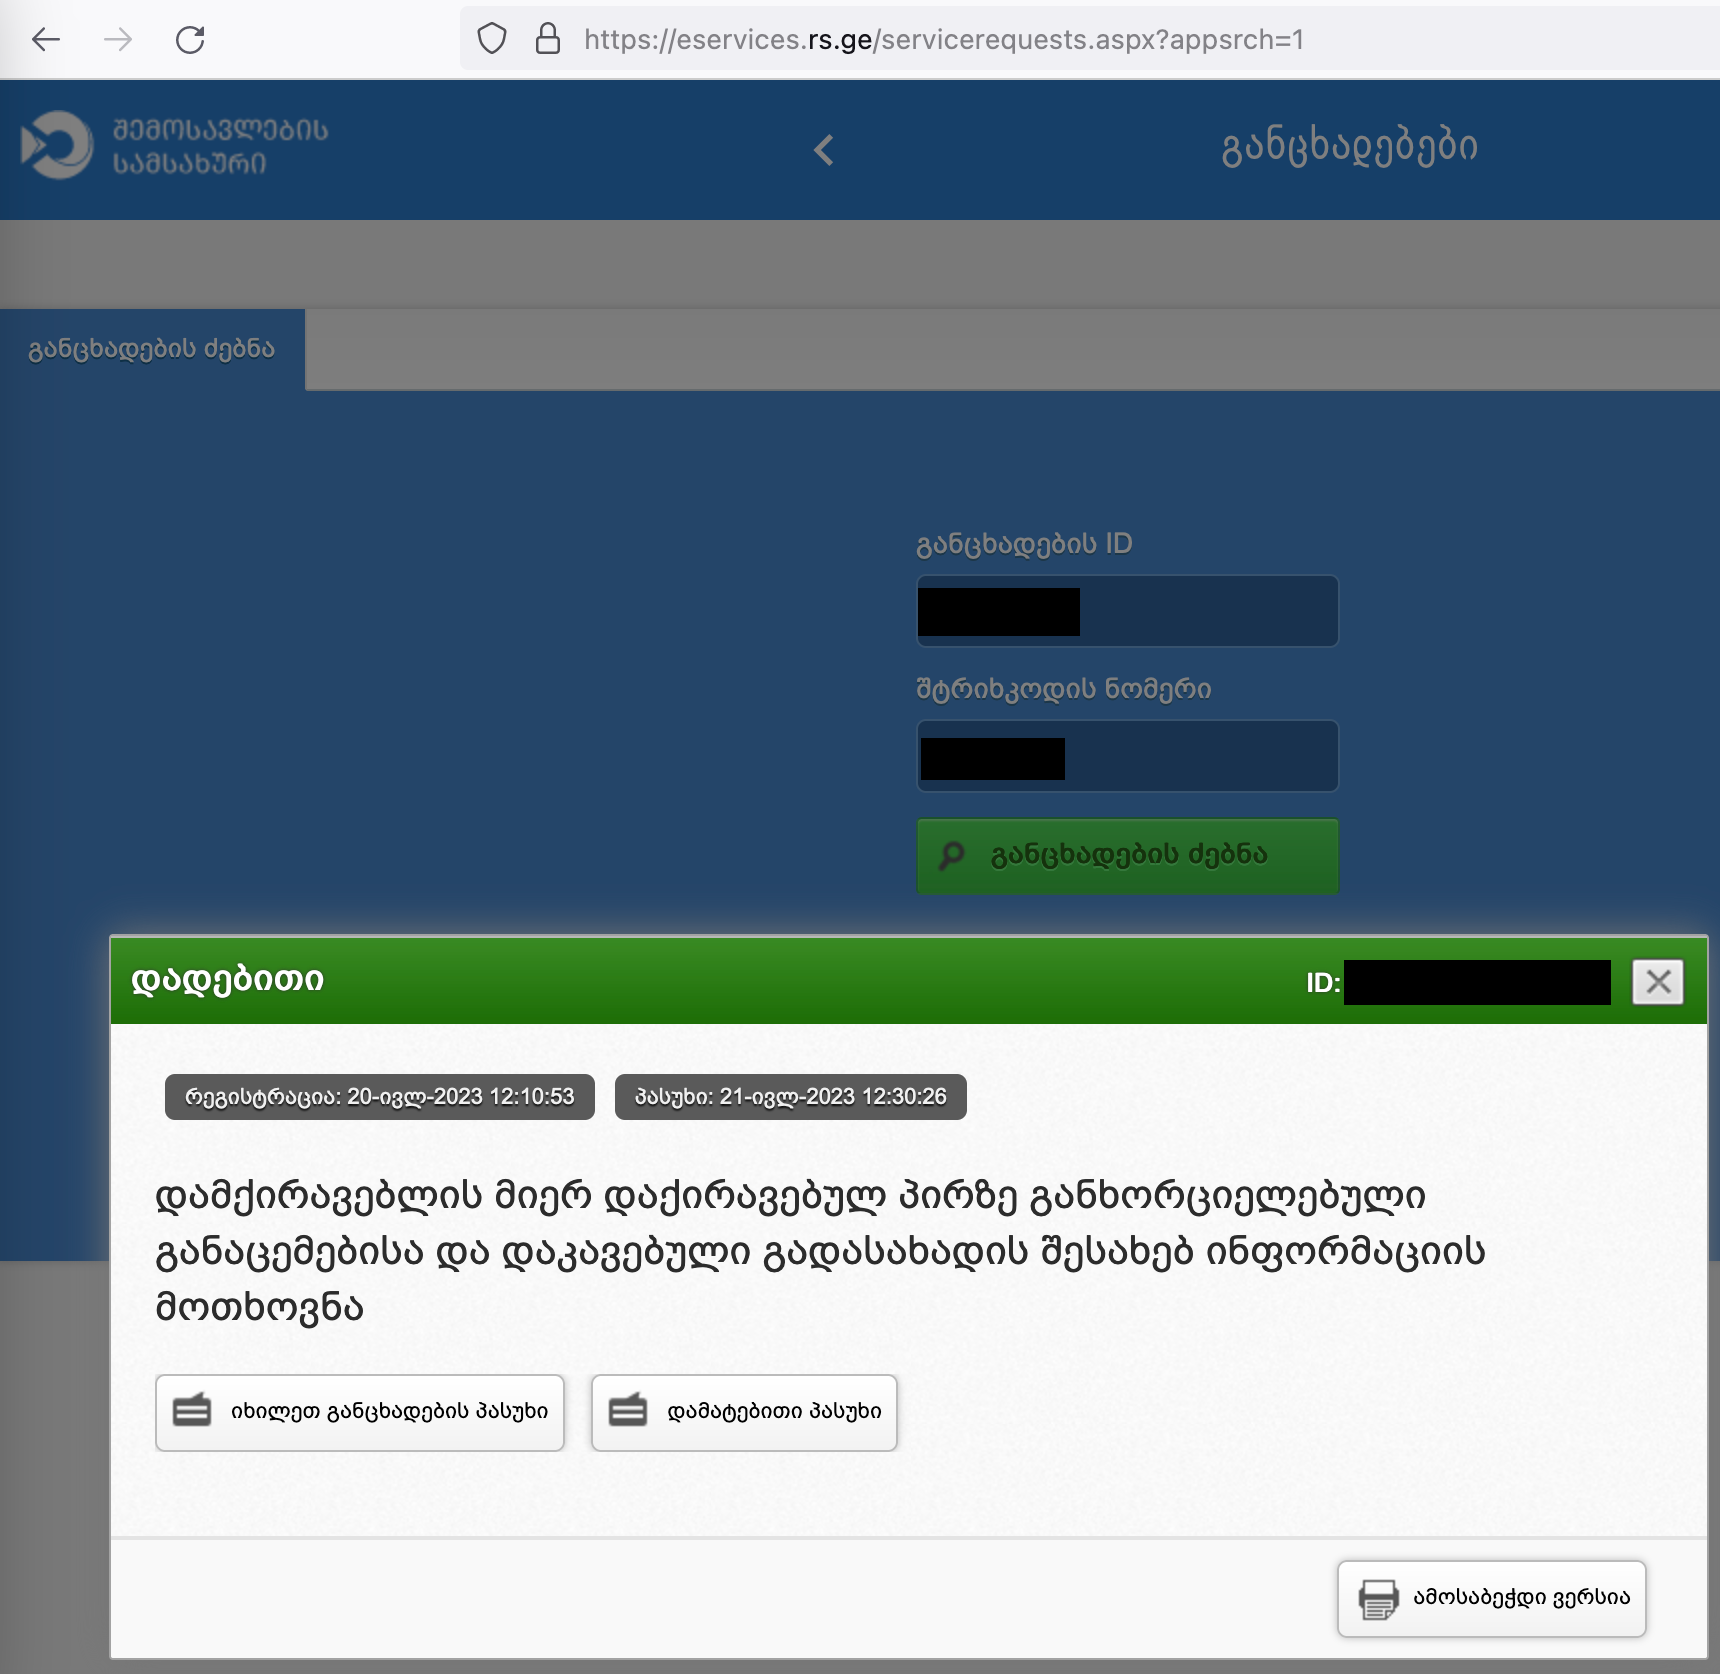
\includegraphics[width=35em]{rs-verification_public}
\end{center}

\pagebreak
